\documentclass[11pt]{report}
\usepackage[spanish]{babel}
\usepackage[utf8]{inputenc}
\usepackage{graphicx}
\usepackage{geometry}
\usepackage{fancyhdr}
\usepackage{amsmath}
\usepackage{helvet}
\usepackage{titlesec}
\usepackage{setspace}
\usepackage{tocloft}
\usepackage{hyperref}
\usepackage{csquotes}
\usepackage{placeins}

\setlength{\parskip}{0.5em}

\usepackage[style=numeric,sorting=none]{biblatex}
\addbibresource{referencias.bib} 

\onehalfspacing
\renewcommand{\familydefault}{\sfdefault}

\geometry{
  letterpaper,
  left=3cm,
  right=2cm,
  top=2.5cm,
  bottom=2cm,
}

\addto\captionsspanish{
  \renewcommand{\contentsname}{Índice}
}
\renewcommand{\cftchapdotsep}{\cftdotsep}  % Para capítulos
\renewcommand{\cftsecdotsep}{\cftdotsep}   % Para secciones
\renewcommand{\cftsubsecdotsep}{\cftdotsep} % Para subsections

\titleformat{\chapter}[display]
  {\normalfont\Large\bfseries}
  {\chaptername\ \thechapter}
  {10pt}
  {\huge}
\titlespacing*{\chapter}{0pt}{-20pt}{20pt}  % Ajusta el espaciado aquí

\begin{document}

% Title page
\begin{titlepage}
	\begin{center}
		
\includegraphics[width=0.4\textwidth]{imagenes/logo_ubb.png}\\
		\normalsize FACULTAD DE INGENIERÍA\\
		DEPTO. INGENIERÍA ELÉCTRICA Y ELECTRÓNICA\\[2cm]

		\LARGE \textbf{``Implementación de un Controlador FOC para Motores Brushless con Encoder Utilizando STM32''}\\[6cm]

		\normalsize AUTOR:\\
		RODRIGO FUENTES PEDREROS\\
		\href{https://www.youtube.com/watch?v=dQw4w9WgXcQ}{\phantom{ASDF}}\\[2cm]

		SEMINARIO PARA OPTAR AL TÍTULO DE\\
		INGENIERO DE EJECUCIÓN EN ELECTRÓNICA\\[1cm]

		CONCEPCIÓN - CHILE\\
		AÑO 2024\\
	\end{center}
\end{titlepage}

% Back title page
\begin{titlepage}
	\begin{center}
		
\includegraphics[width=0.4\textwidth]{imagenes/logo_ubb.png}\\
		\normalsize FACULTAD DE INGENIERÍA\\
		DEPTO. INGENIERÍA ELÉCTRICA Y ELECTRÓNICA\\[2cm]

		\LARGE \textbf{``Implementación de un Controlador FOC para Motores Brushless con Encoder Utilizando STM32''}\\[5cm]

		\normalsize AUTOR\\
		RODRIGO FUENTES PEDREROS\\[3cm]

		\large PROFESOR GUÍA:\\
		\large ANGEL ERNESTO RUBIO\\[1cm]
		\large PROFESORES GUÍA ADJUNTO:\\
		\large PEDRO MELIN COLINA
	\end{center}
\end{titlepage}

\normalsize
\pagenumbering{arabic}
\setcounter{page}{3}

\newpage
\tableofcontents

%\newpage
%\listoffigures

%\newpage
%\listoftables

\newpage
\chapter*{Resumen}
\addcontentsline{toc}{chapter}{Resumen}

\newpage
\chapter{Introducción}
\section{Introducción general}
Cuando se habla de motores eléctricos de corriente continua, los motores sin escobillas destacan por su alto desempeño, siendo la opción preferida en aplicaciones como vehículos eléctricos, drones, robótica avanzada y robótica industrial.

Para los motores \textit{brushless}, existe una gran variedad de técnicas de control. Algunas de las más relevantes son el control trapezoidal, utilizado mayormente en drones; el control directo de torque (DTC), empleado principalmente en motores de media y alta potencia; y el control FOC, que se aplica mayormente en robótica. En este documento, se tratará únicamente esta última técnica.

Existen tres aspectos clave que diferencian cada técnica: el rizado de torque, el costo computacional y la complejidad del hardware necesario para su ejecución. En estos aspectos, el control FOC es uno de los que produce menor rizado de torque, aunque requiere un mayor coste computacional y hardware especializado.

Este proyecto presenta la implementación y validación de un controlador de campo orientado (FOC) para motores sin escobillas de corriente continua (BLDC). Se desarrolló la placa controladora utilizando STM32 y se implementó el algoritmo de control FOC en lenguaje C.

\newpage
\section{Marco teórico}
\subsection{Motores \textit{brushless}}
Los motores \textit{brushless} (BLDC), o motores sin escobillas de corriente continua, son dispositivos en los que el embobinado se encuentra en el estátor, mientras que el rotor contiene los imanes permanentes.

Estos motores se destacan por ofrecer una mayor densidad de potencia en comparación con los motores de escobillas. Sin embargo, dicha ventaja implica una mayor complejidad, ya que requieren un controlador electrónico que se encargue de la conmutación de las fases del embobinado para generar el movimiento del rotor.

Los motores \textit{brushless} tienen tres fases que pueden ser energizadas de manera positiva o negativa, lo que genera ocho posibles configuraciones de polarización. De estas, dos son configuraciones nulas, lo que deja seis combinaciones útiles para el control del movimiento. Estas seis configuraciones son la base de uno de los métodos de control más sencillos, conocido como control trapezoidal o de seis pasos. Este método se limita a conmutar las seis polarizaciones en secuencia para completar un ciclo de rotación. No obstante, este enfoque sacrifica eficiencia y produce un rizado de torque considerable \cite{fisher2014high_STEP} \cite{juanpere_tecnicas}.

\newpage
\subsection{Control Orientado de Campo (FOC)}
El control FOC es una de las técnicas más utilizadas para el control de motores \textit{brushless} en robótica, debido a que ofrece una alta eficiencia, un bajo rizado de torque y una gran precisión en el control del motor \cite{Garca2011ComparisonBF}\cite{juanpere_tecnicas}.

\begin{figure}[ht]
    \centering
    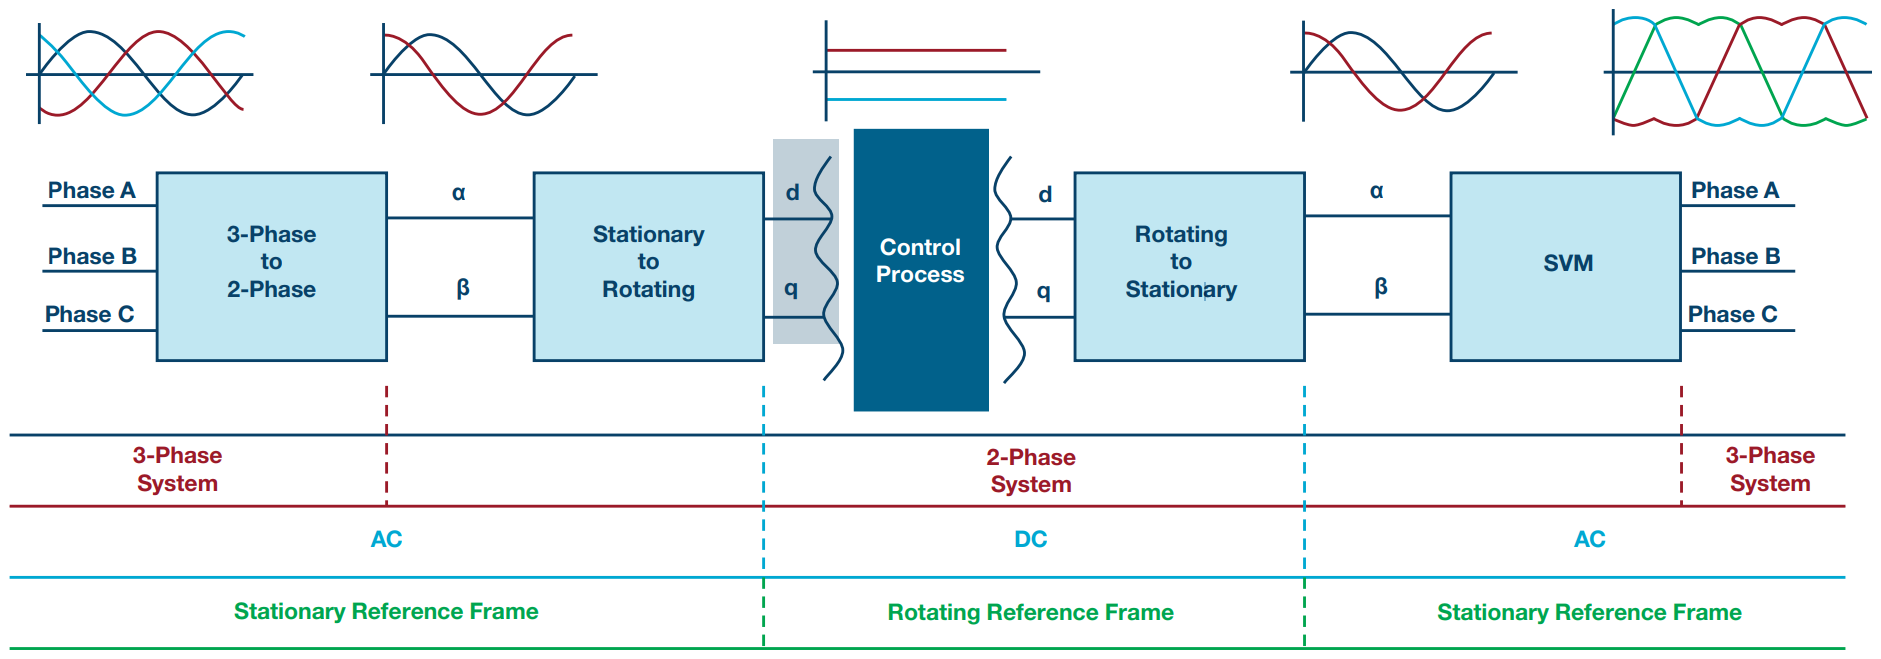
\includegraphics[width=0.8\textwidth]{imagenes/transformadas_foc.png}
    \caption{Esquema de transformadas en FOC \cite{frick2018bldc}.}
    \label{fig:foc_transform}
\end{figure}
\FloatBarrier

Esta técnica se basa en la transformación de las variables trifásicas del motor, que se encuentran en un marco de referencia estático, hacia un marco de referencia rotacional que gira de manera síncrona con el rotor del motor. Al realizar esta transformación, es posible convertir variables que tienen un comportamiento ondulatorio en el tiempo en variables con un comportamiento lineal. Esto se logra mediante la aplicación de la transformada de Clarke y la transformada de Park.

\newpage
\subsection{Transformada de Clarke}
La transformada de Clarke convierte un sistema trifásico de corrientes \(ABC\) en un sistema bifásico \(\alpha-\beta\), proyectando las corrientes en un sistema de coordenadas bidimensional estacionario \cite{AN1078}.

\begin{figure}[ht]
    \centering
    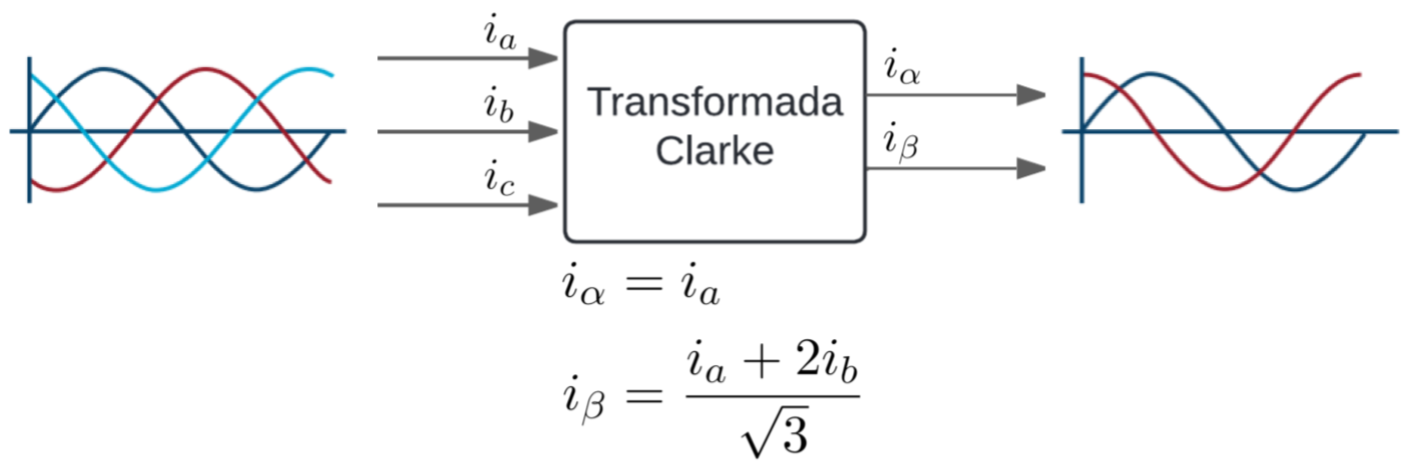
\includegraphics[width=0.5\textwidth]{imagenes/clarke.png}
    \caption{Transformada de Clarke \cite{AN1078}.}
    \label{fig:clarke_transform}
\end{figure}
\FloatBarrier

\subsection{Transformada de Park}
La transformada de Park convierte el sistema estacionario \(\alpha-\beta\) en un sistema rotatorio \(dq\), sincronizado con el rotor. Esto simplifica el análisis y control del motor al reducir la complejidad de las señales del motor \cite{AN1078}.

\begin{figure}[ht]
    \centering
    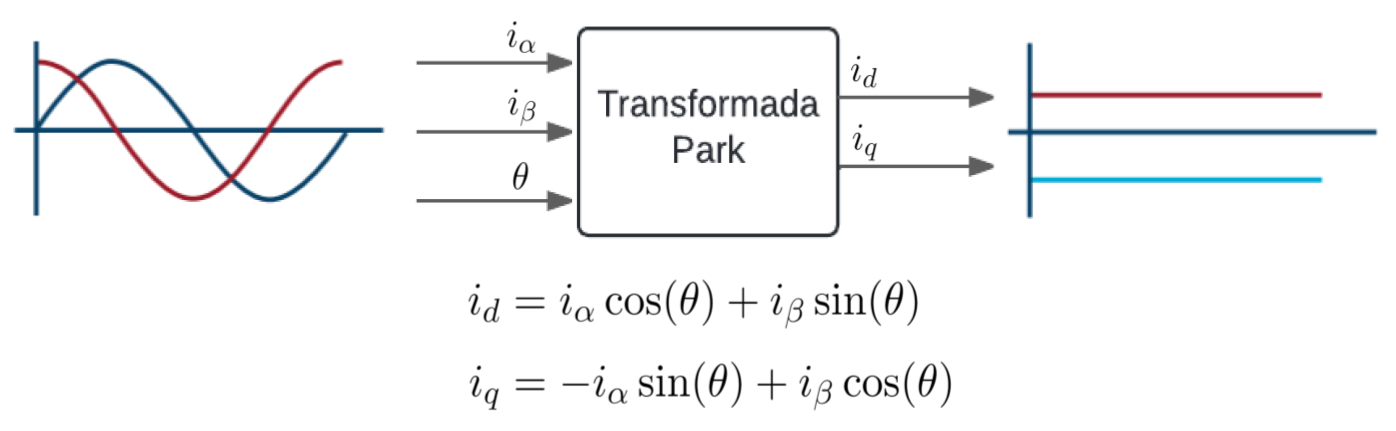
\includegraphics[width=0.5\textwidth]{imagenes/park.png}
    \caption{Transformada de Park \cite{AN1078}.}
\end{figure}
\FloatBarrier

\subsection{Transformada inversa de Park}
La transformada inversa de Park regresa el sistema rotatorio \(dq\) al marco estacionario \(\alpha-\beta\), permitiendo aplicar las señales de control al motor en su forma original \cite{AN1078}.

\begin{figure}[ht]
    \centering
    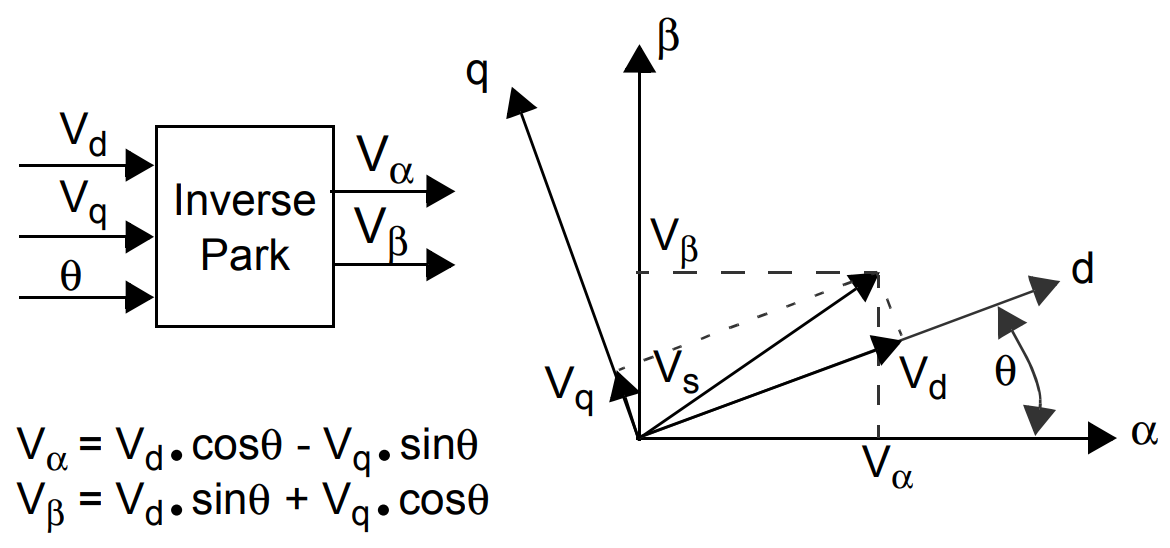
\includegraphics[width=0.5\textwidth]{imagenes/park_inv.png}
    \caption{Transformada inversa de Park \cite{AN1078}.}
\end{figure}
\FloatBarrier


\subsection{Modulación de Espacio Vectorial (SVM)}
La modulación de espacio vectorial es una técnica que busca obtener los tiempos de activación para cada embobinado del motor con el fin de ‘sintetizar’ un vector intermedio en el campo electromagnético del estátor.

\begin{figure}[ht]
	\centering
	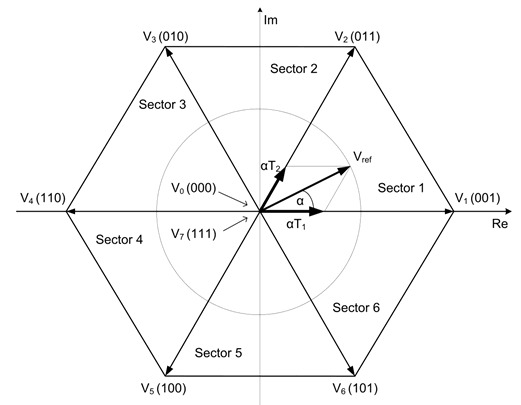
\includegraphics[width=0.5\textwidth]{imagenes/image909-0000.jpg}
	\caption{SVM.}
\end{figure}
\FloatBarrier

\newpage
\section{Motivación}
Este proyecto nace de la necesidad de un controlador para motores brushless adecuado para su uso en robots de competencia en la categoría de robot sumo autónomo. En esta categoría, este tipo de motores no son normalmente utilizados debido a las limitaciones de los controladores comerciales y los riesgos que conlleva la sobrecarga de los motores en periodos cortos de acción, ya que los controladores comerciales no están pensados para esto.

\section{Objetivos}
\subsection{Objetivo General}
Implementar un controlador de tipo FOC (Control de Campo Orientado) para motores brushless con encoder, utilizando un microcontrolador STM32, que sirva de base para un driver especializado en la robótica competitiva.

\subsection{Objetivos Específicos}
\begin{itemize}
	\item Estudiar los principios del Control de Campo Orientado (FOC) y la modulación de espacio vectorial (SVM) para aplicarlos en el diseño del controlador.
	\item Diseñar el hardware para el controlador FOC, con los componentes mínimos necesarios para validar el funcionamiento.
	\item Configurar y programar el microcontrolador para el algoritmo FOC, utilizando las librerías HAL de STM32
	\item Validar el funcionamiento del controlador y proponer posibles mejoras para su aplicación en robótica competitiva.
\end{itemize}

\newpage
\subsection{Alcances}
\begin{itemize}
	\item Se configurará el microcontrolador utilizando STM32CubeMX.
	\item Se implementará el controlador de velocidad y corriente.
	\item No se implementará el control de posición.
	\item Se programará el firmware utilizando VScode y el lenguaje C.
	\item El firmware se compilará utilizando un makefile y GCC, junto con la extensión STM32 en VScode.
	\item Se cargará el firmware utilizando STM32CubeProgrammer y ST-link.
	\item Se diseñará la PCB en Eagle.
	\item Se diseñarán las piezas adicionales en Autodesk Inventor, para su posterior fabricación mediante impresión 3D.
	\item La PCB se fabricará y semi ensamblará utilizando JLCPCB.
	\item Se obtendrán datos detallados durante el tiempo de ejecución.
	\item Los datos se graficarán utilizando Plotly en Python.
	\item Se identificarán posibles mejoras.
\end{itemize}

%la idea es que haya una correlación, entre los capítulos, esto es la documentación del poseso para llegar a un objetivo
%si se desarrolla algo, se debe fundamentar en el marco teórico, diseñar en la implementación y posteriormente validarlo
%la idea es que no hayan cosas sueltas

%la idea de este capitulo es hacer el diseño conceptual del controlador
\chapter{Desarrollo del controlador}
\section{parámetros de diseño}
\subsection{Parámetros del Motor}
\subsection{Microcontrolador}



%la idea de este capitulo es documentan el diseño duro del sistema
\chapter{Diseño de implementación}
\section{hardware}
\section{software}

\chapter{Validación}
Para las validaciones, se realizó una adquisición de datos, donde estos se recopilan ciclo a ciclo en la memoria RAM del microcontrolador para su posterior envío de forma asincrónica por el puerto USB, como se muestra en la figura \ref{flujo_debug}. Los datos son recibidos en una computadora a través de un código en Python, donde se almacenan en archivos CSV. Esta recopilación de información se realiza al final de cada ejecución de la interrupción del sistema, la cual se ejecuta a una frecuencia de 48 kHz. Debido a las limitaciones de memoria, la recopilación de datos solo puede llevarse a cabo durante un período de aproximadamente 100 ms, hasta alcanzar la capacidad máxima de la memoria.

\begin{figure}[ht]
	\centering
	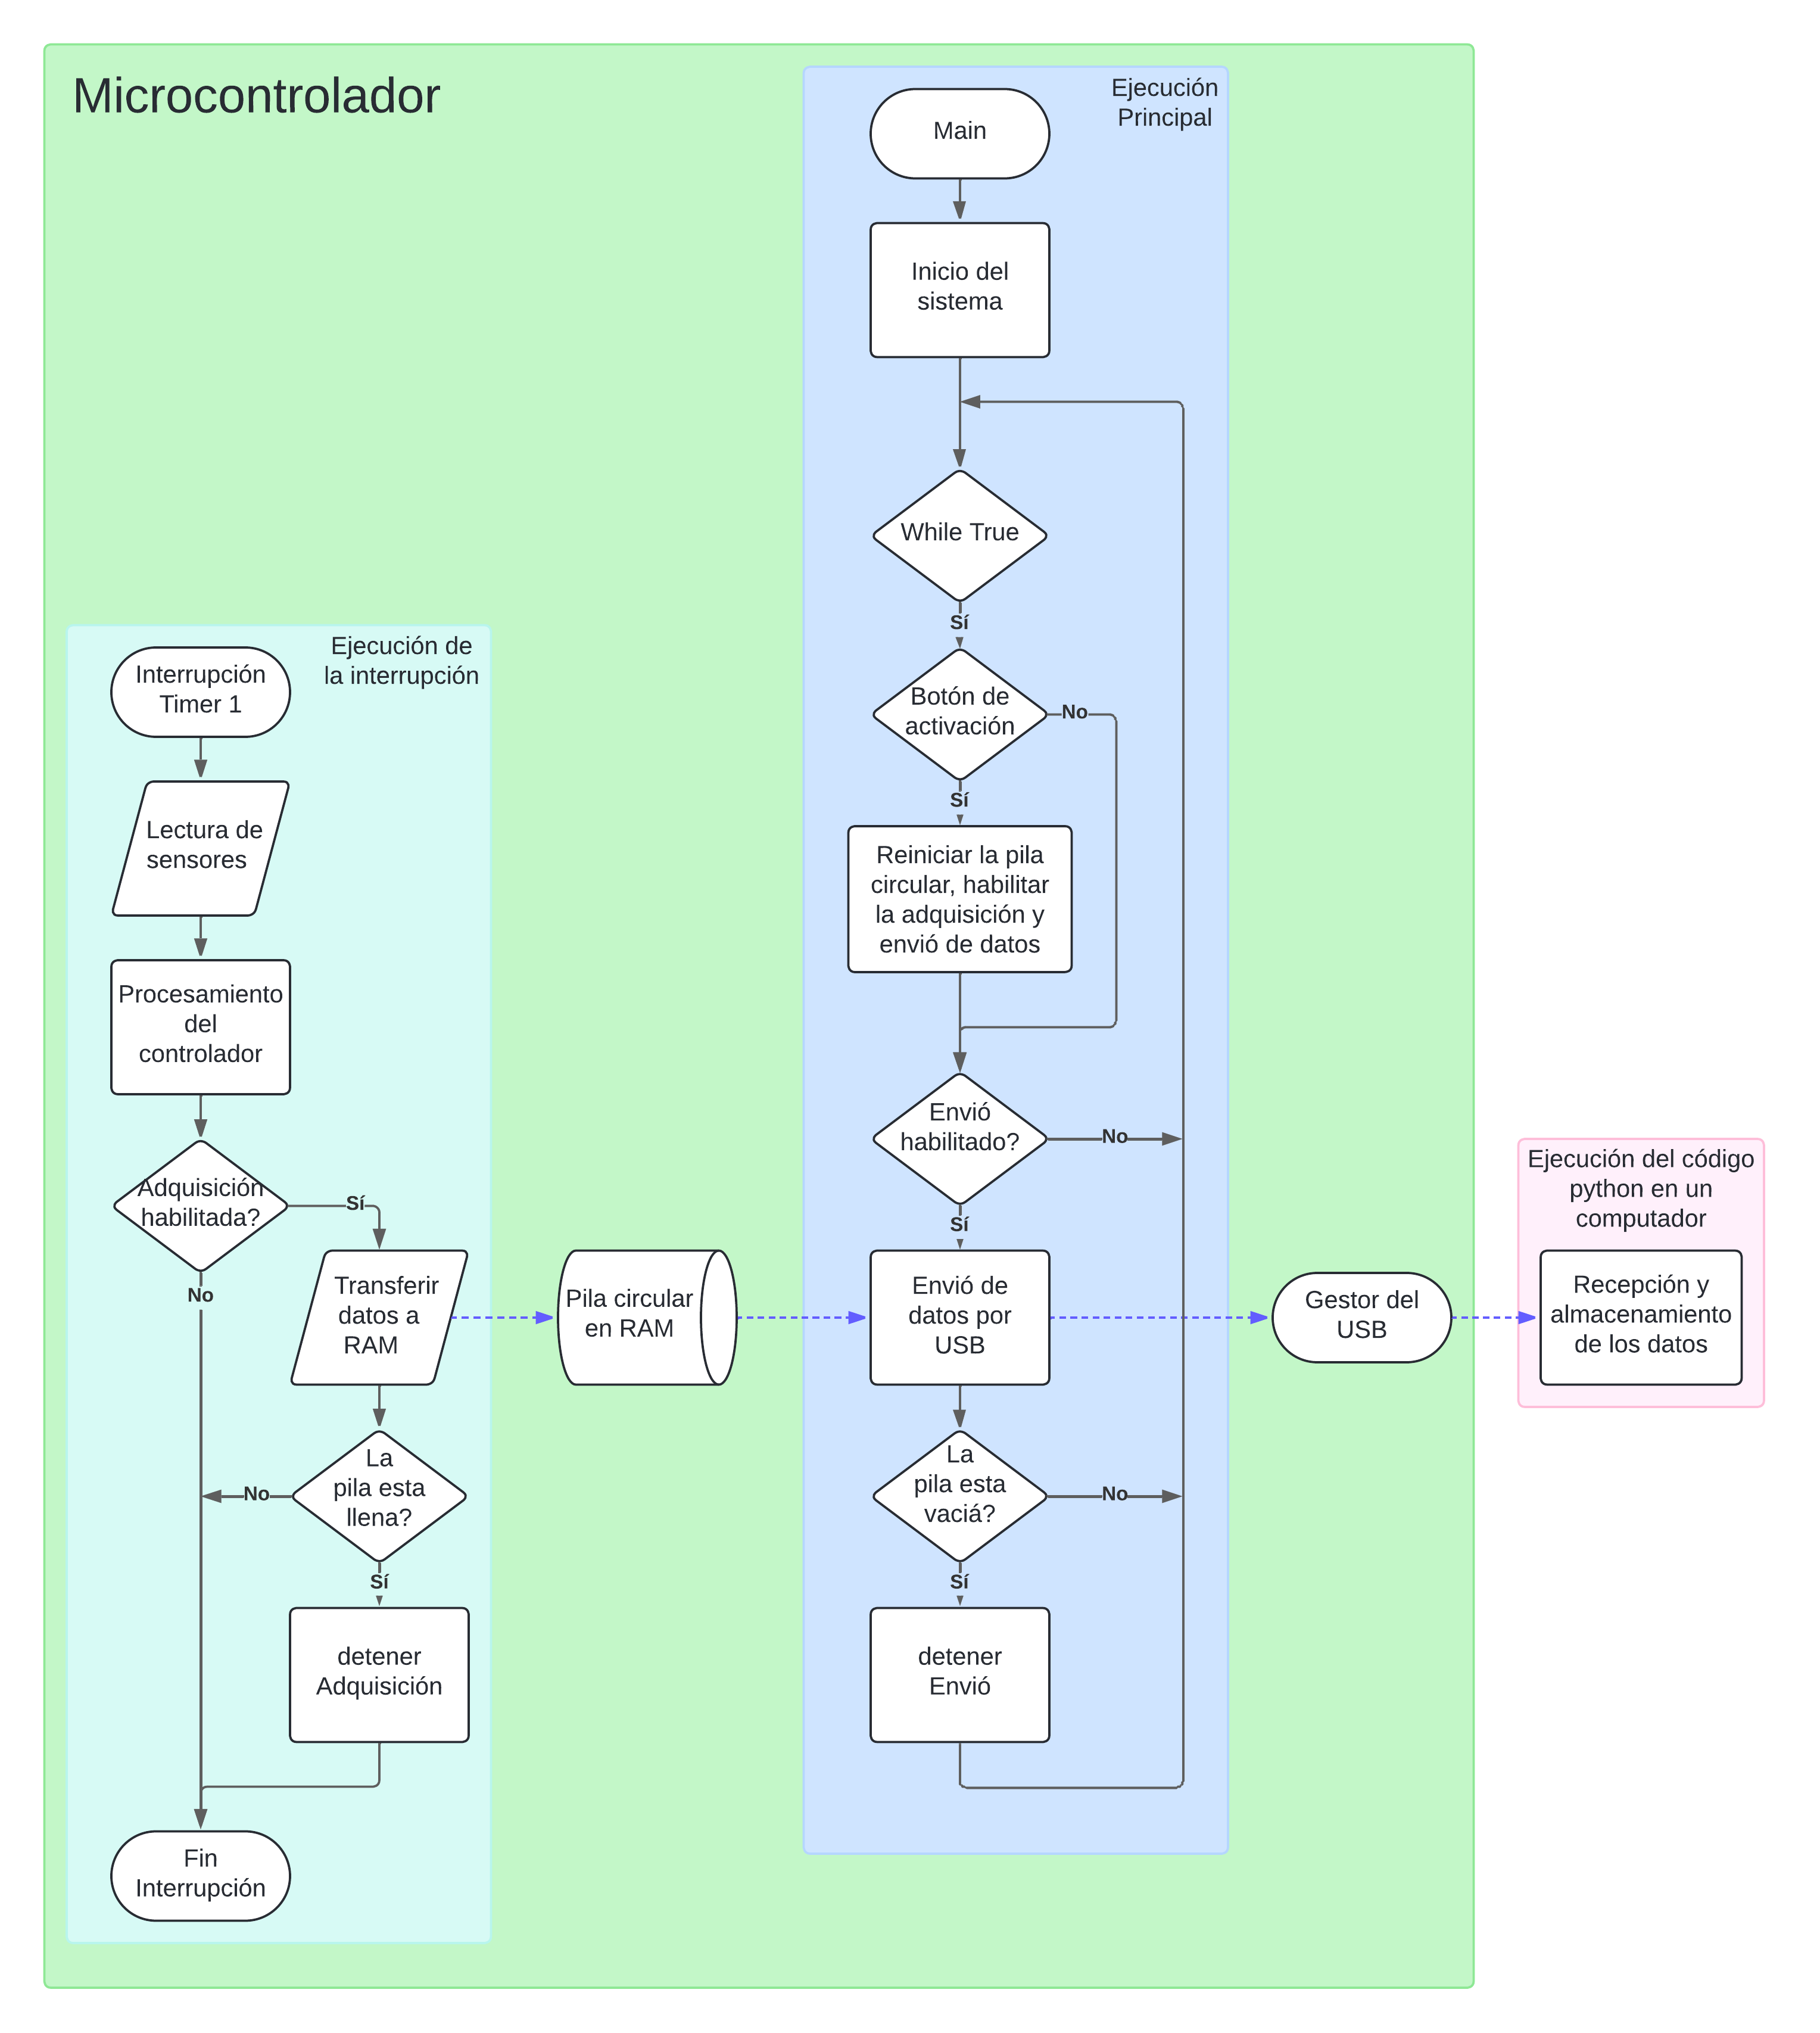
\includegraphics[width=0.8\textwidth]{imagenes/Debug USB.png}
	\caption{Diagrama de flujo adquisición de datos.}
	\label{flujo_debug}
\end{figure}
\FloatBarrier

\section{Validación de la adquisición y transformación de las mediciones de corriente}

\subsection{Validación de las mediciones de corriente}
Se validaran las mediciones de corriente adquiridas desde el microcontrolador.

\begin{figure}[ht]
	\centering
	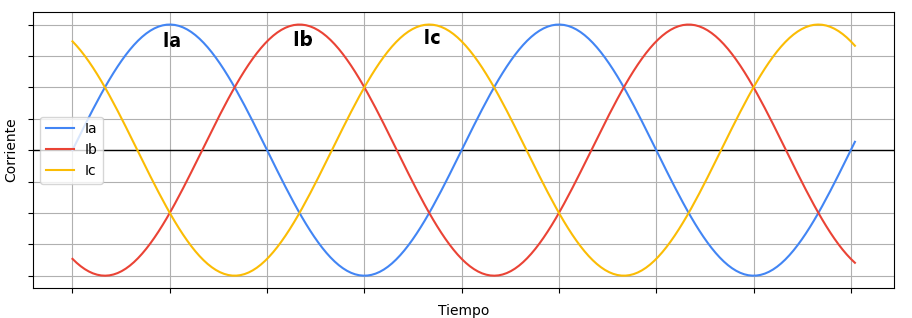
\includegraphics[width=0.8\textwidth]{imagenes/Corrientes_ABC_ideal.png}
	\caption{Corrientes ideales en un sistema trifásico equilibrado.}
	\label{corrientes_ABC_ideal}
\end{figure}
\FloatBarrier

En la figura \ref{corrientes_ABC_ideal} se representan las señales ideales de un sistema trifásico equilibrado, con las tres corrientes de fase $I_a$, $I_b$ e $I_c$, cada una de ellas con una forma senoidal pura y un desfase de $120^\circ$ entre sí.

\begin{figure}[ht]
	\centering
	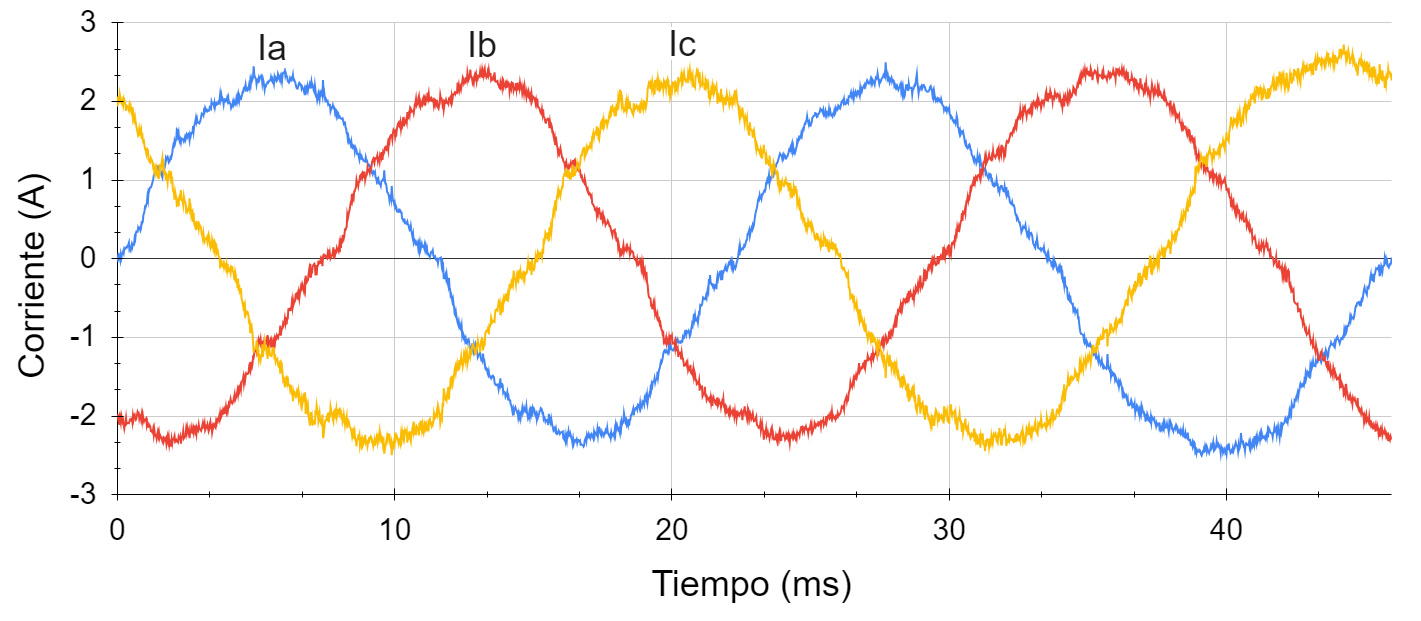
\includegraphics[width=0.8\textwidth]{imagenes/Corrientes_ABC.png}
	\caption{Corrientes medidas en el sistema trifásico.}
	\label{corrientes_ABC}
\end{figure}
\FloatBarrier

En la figura \ref{corrientes_ABC} se pueden apreciar las corrientes de fase, las cuales presentan una cantidad significativa de ruido, aun cuando internamente pasan por un filtro complementario con una frecuencia de corte $f_W=12000Hz$, pero mantienen un comportamiento sinusoidal con el desfase de $120^\circ$ entre señales, como es característico de un sistema trifásico equilibrado. pero la cantidad de ruido podría indicar que seria necesario disminuir la frecuencia de corte en el filtro complementario o agregar un filtro pasivo en el circuito.

\newpage
\subsection{Validación de la transformada de Clarke}

Se validara los resultado a la salida de la transformada de Clarke en el microcontrolador.

\begin{figure}[ht]
	\centering
	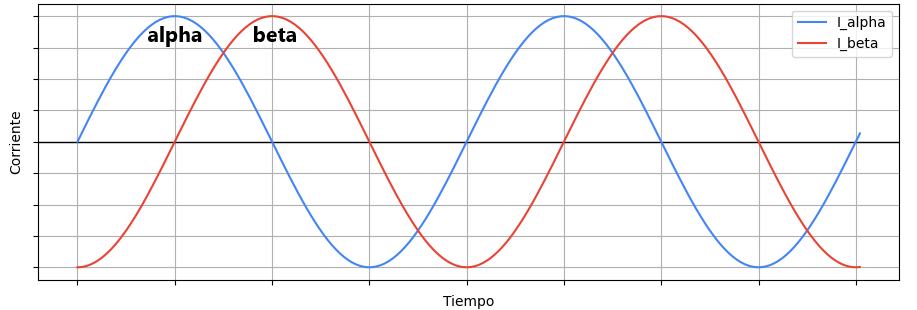
\includegraphics[width=0.8\textwidth]{imagenes/Corrientes_AlphaBeta_ideal.png}
	\caption{Corrientes ideales en el plano $\alpha\beta$.}
	\label{corrientes_alpha_beta_ideal}
\end{figure}
\FloatBarrier

En la figura \ref{corrientes_alpha_beta_ideal} se representan las corrientes ideales en el plano $\alpha\beta$, con las formas senoidales puras con un desfase de $90^\circ$ entre sí.

\begin{figure}[ht]
	\centering
	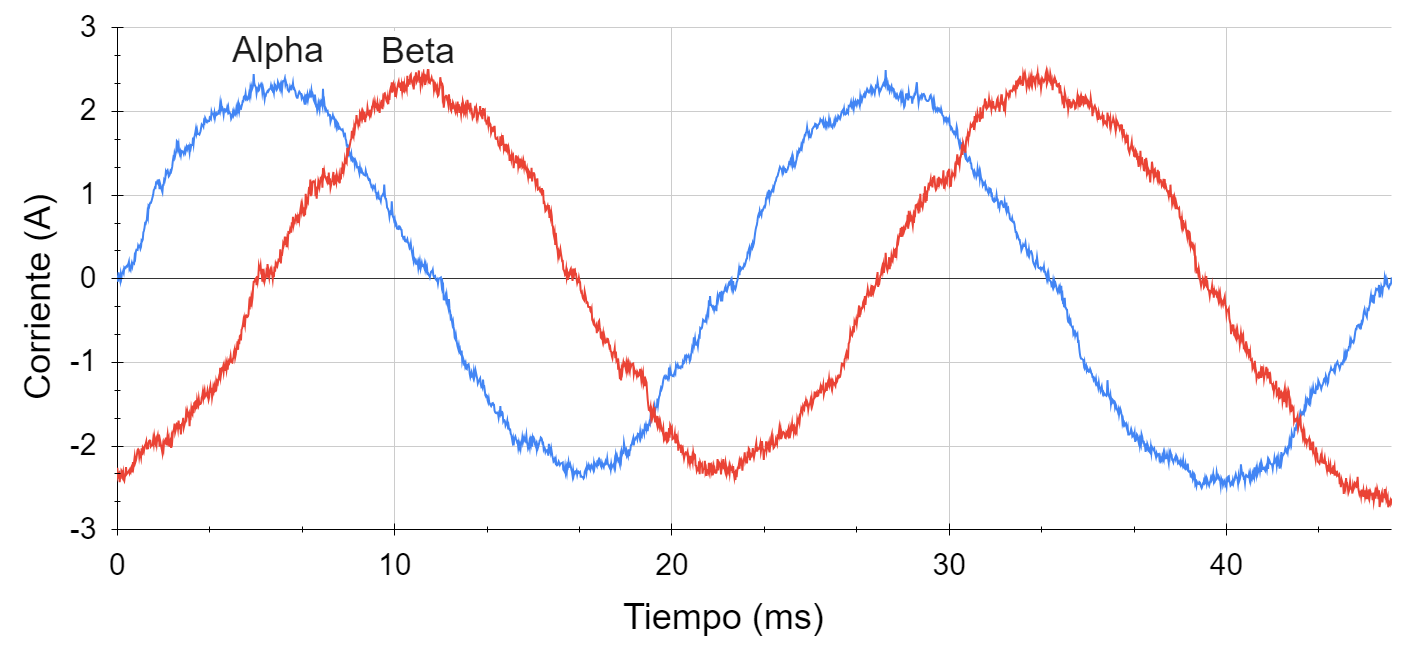
\includegraphics[width=0.8\textwidth]{imagenes/Corrientes_AlphaBeta.png}
	\caption{Corrientes medidas en el plano $\alpha\beta$.}
	\label{corrientes_alpha_beta}
\end{figure}
\FloatBarrier

En la figura \ref{corrientes_alpha_beta} se pueden apreciar como las corrientes $\alpha\beta$ reflejan el ruido presente en las mediciones de los sensores de corriente, pero mantienen un comportamiento esperado a la salida de la transformada de Clarke con las dos señales sinusoidal con el desfase de $90^\circ$ entre señales, como es característico.

\newpage
\subsection{Validación de la transformada de Park}

Se validara los resultado a la salida de la transformada de Park en el microcontrolador.

\begin{figure}[ht]
	\centering
	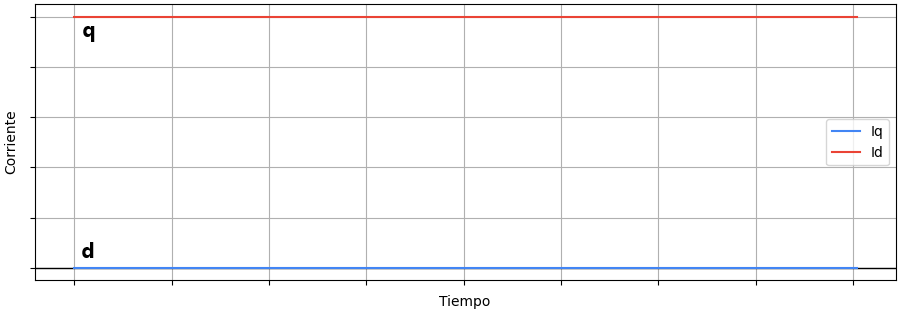
\includegraphics[width=0.8\textwidth]{imagenes/Corrientes_dq_ideal.png}
	\caption{Corrientes ideales en el plano $dq$.}
	\label{corrientes_dq_ideal}
\end{figure}
\FloatBarrier

En la figura \ref{corrientes_dq_ideal} se representan las corrientes ideales en el plano $dq$, donde lo ideal, es que la corriente directa tenga un valor de cero, para mantener la eficiencia del sistema, mientras que solo la corriente de cuadratura tiene un valor distinto a cero.

\begin{figure}[ht]
	\centering
	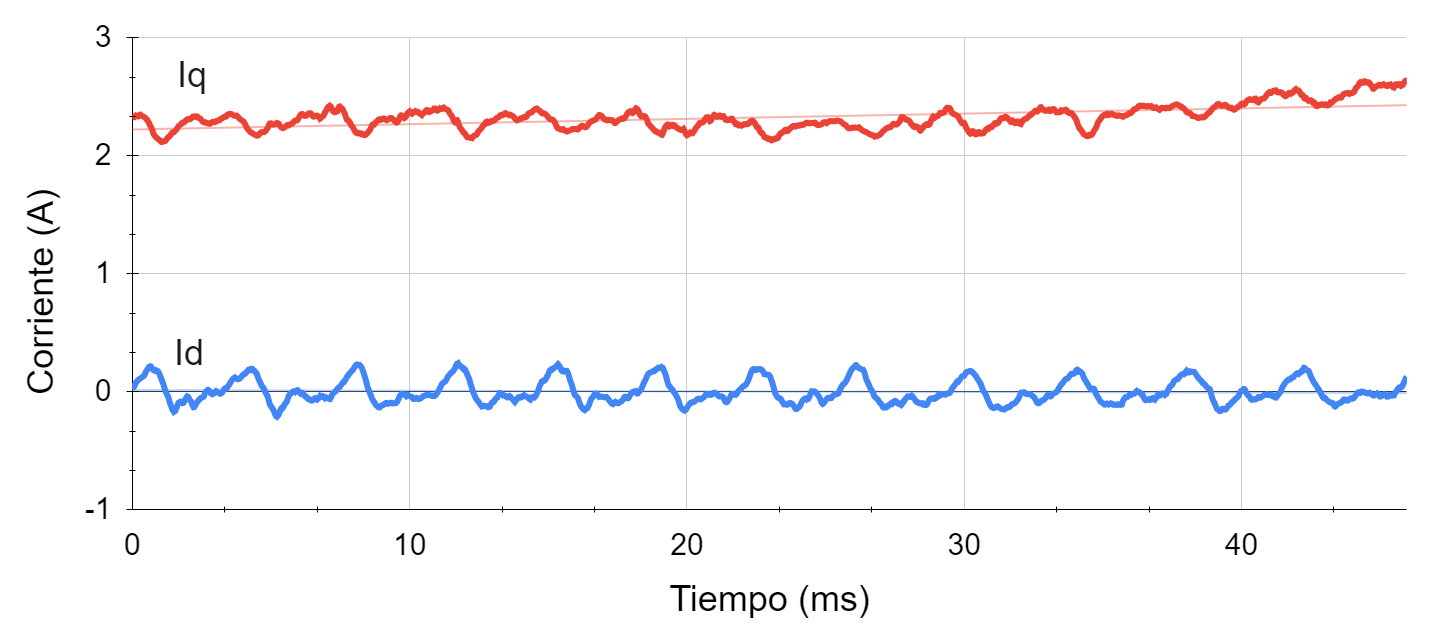
\includegraphics[width=0.8\textwidth]{imagenes/Corrientes_dq.png}
	\caption{Corrientes medidas en el plano $dq$.}
	\label{corrientes_dq}
\end{figure}
\FloatBarrier

En la figura \ref{corrientes_dq} se pueden apreciar como las corrientes $dq$ presenta una menor cantidad de ruido gracias a que su filtro complementario esta ajustado para una frecuencia de corte de $f_W=800Hz$, aunque igualmente presentan ciertas deformaciones y e inestabilidad con un patron aparentemente constante, pero en términos generales mantienen aproximadamente el comportamiento esperado a la salida de la transformada de Park.

\newpage
\section{Validación de los Controladores PI}
En esta validación se quiere ver si los controladores PI de velocidad y corriente son capaces de mantener sus set point. estas pruebas se realizaron de forma estática, aplicando un poco de carga sobre el motor y tomando una captura de datos durante esto.

\subsection{Validación del controlar de velocidad}
Para la validación se aplico un set point de 116.8 RPM con uno de los potenciómetros.

\begin{figure}[ht]
	\centering
	\includegraphics[width=0.8\textwidth]{ruta/del/primer_grafico.png}
	\caption{Velocidad medida por el encoder y setpoint de velocidad.}
	\label{velocidad_encoder}
\end{figure}
\FloatBarrier

\subsection{Validación del controlar de corriente}

\section{Validación señales de Modulación}
%aquí seria mejor comparar respecto a datos obtenidos con un analizador lógico

\newpage
\section{Validación de los Controladores PI}
En esta validación se busca comprobar si los controladores PI de velocidad y corriente son capaces de mantener sus setpoints. Las pruebas se realizaron de forma estática, aplicando una carga ligera sobre el motor y capturando datos durante este proceso.

\subsection{Validación del controlador de velocidad}
Para la validación, se aplicó un setpoint de 116.8 RPM utilizando uno de los potenciómetros disponibles.

\begin{figure}[ht]
	\centering
	\includegraphics[width=0.8\textwidth]{ruta/del/primer_grafico.png}
	\caption{Velocidad medida por el encoder y setpoint de velocidad.}
	\label{velocidad_encoder}
\end{figure}
\FloatBarrier

En la Figura \ref{velocidad_encoder}, se observa que la velocidad medida por el encoder sigue adecuadamente el setpoint establecido de 116.8 RPM. A pesar de ligeras oscilaciones, el controlador de velocidad mantiene el régimen deseado, demostrando su capacidad para alcanzar y mantener el setpoint bajo condiciones de carga estática.

\subsection{Validación del controlador de corriente}

\begin{figure}[ht]
	\centering
	\includegraphics[width=0.8\textwidth]{ruta/del/segundo_grafico.png}
	\caption{Corrientes medidas en el plano $dq$.}
	\label{corrientes_dq}
\end{figure}
\FloatBarrier

Como se muestra en la Figura \ref{corrientes_dq}, las corrientes en el plano $dq$ indican que el controlador de corriente logra mantener la corriente de cuadratura ($I_q$) cercana al valor de referencia proporcionado por el controlador de velocidad, mientras que la corriente directa ($I_d$) se mantiene próxima a cero. Esto evidencia que el controlador de corriente regula eficazmente las corrientes según los setpoints establecidos.

\begin{figure}[ht]
	\centering
	\includegraphics[width=0.8\textwidth]{ruta/del/tercer_grafico.png}
	\caption{Voltajes en el plano $dq$.}
	\label{voltajes_dq}
\end{figure}
\FloatBarrier

Además, la Figura \ref{voltajes_dq} presenta los voltajes en el plano $dq$, donde se aprecia que las tensiones generadas están dentro de los valores esperados para mantener las corrientes deseadas. Esto corrobora que el controlador de corriente responde adecuadamente a las demandas del sistema, contribuyendo al correcto desempeño del motor bajo condiciones de carga.

\newpage
\chapter*{Comentarios y Conclusiones}
\addcontentsline{toc}{chapter}{Comentarios y Conclusiones}

\newpage
\addcontentsline{toc}{chapter}{Bibliografía}
\printbibliography

\newpage
\addcontentsline{toc}{chapter}{Anexos}

\chapter*{Anexo A}
\addcontentsline{toc}{section}{Anexo A}

\end{document}
